\documentclass[11pt,a4paper]{article}
\usepackage[a4paper,margin=2cm]{geometry}
\usepackage[T1]{fontenc}
\usepackage[utf8]{inputenc}
\usepackage{lmodern}
\usepackage{microtype}
\usepackage{amsmath}
\usepackage{graphicx}
\usepackage{booktabs}
\usepackage{array}
\usepackage{longtable}
\usepackage{placeins}
\usepackage{caption}
\usepackage[numbers,sort&compress]{natbib}
\usepackage{xurl}
\usepackage[hidelinks]{hyperref}
\usepackage{xcolor}
\usepackage{indentfirst}
\captionsetup{font=small,labelfont=bf,skip=4pt}
\setlength{\parskip}{2pt}
\setlength{\parindent}{1.5em}
\setlength{\bibsep}{1pt}
\setlength{\emergencystretch}{3em}
% Generated numerical definitions from this run.
% Auto-generated by scripts/05_figures_tables.py from results/*.json. Do not edit.
\newcommand{\AUCciCART}{[0.739, 0.780]}
\newcommand{\AUCciLR}{[0.773, 0.812]}
\newcommand{\AUCciXGB}{[0.777, 0.815]}
\newcommand{\AgreeCARTXGB}{89.7\%}
\newcommand{\AgreeLRCART}{88.3\%}
\newcommand{\AgreeLRXGB}{94.2\%}
\newcommand{\AllNineBadRate}{54.9\%}
\newcommand{\BadRateMDENever}{39.8\%}
\newcommand{\BadRateMDEOneTwenty}{62.4\%}
\newcommand{\BadRatePop}{52.0\%}
\newcommand{\BgBaseSDFiftyXGB}{0.139}
\newcommand{\BgBaseSDTwoXGB}{0.088}
\newcommand{\BrierciCART}{[0.1912, 0.2097]}
\newcommand{\BrierciLR}{[0.1767, 0.1942]}
\newcommand{\BrierciXGB}{[0.1752, 0.1929]}
\newcommand{\CARTccp}{0.0005}
\newcommand{\CARTdepth}{5}
\newcommand{\CARTleaves}{18}
\newcommand{\CARTleavesMax}{19}
\newcommand{\CARTleavesMin}{16}
\newcommand{\CARTminleaf}{200}
\newcommand{\CARTpath}{4.4}
\newcommand{\CARTrootTop}{ExternalRiskEstimate}
\newcommand{\CARTrootTopN}{30}
\newcommand{\CARTvars}{6}
\newcommand{\CITLCART}{+0.006}
\newcommand{\CITLLR}{+0.005}
\newcommand{\CITLXGB}{+0.006}
\newcommand{\CVAUCCART}{0.781}
\newcommand{\CVAUCCARTdepthTwo}{0.757}
\newcommand{\CVAUCLR}{0.806}
\newcommand{\CVAUCXGB}{0.809}
\newcommand{\CVBrierCART}{0.1896}
\newcommand{\CVBrierLR}{0.1791}
\newcommand{\CVBrierXGB}{0.1778}
\newcommand{\CalSlopeCART}{0.83}
\newcommand{\CalSlopeLR}{0.95}
\newcommand{\CalSlopeXGB}{0.96}
\newcommand{\CaseDCART}{0.22}
\newcommand{\CaseDLR}{0.65}
\newcommand{\CaseDLeaf}{581}
\newcommand{\CaseDXGB}{0.71}
\newcommand{\CaseSAvgMInFile}{383}
\newcommand{\CaseSCART}{0.79}
\newcommand{\CaseSLR}{0.47}
\newcommand{\CaseSLRAvg}{$-$2.34}
\newcommand{\CaseSLeaf}{342}
\newcommand{\CaseSMissingSplits}{4}
\newcommand{\CaseSNSpecial}{9}
\newcommand{\CaseSPathLen}{5}
\newcommand{\CaseSXGB}{0.74}
\newcommand{\CaseSXGBAvg}{$-$0.32}
\newcommand{\CaseTCART}{0.49}
\newcommand{\CaseTLR}{0.50}
\newcommand{\CaseTLeaf}{307}
\newcommand{\CaseTXGB}{0.51}
\newcommand{\ConflictBgFiftyLR}{11.3\%}
\newcommand{\ConflictBgFiftyXGB}{4.6\%}
\newcommand{\ConflictBgTwoXGB}{1.8\%}
\newcommand{\ConflictRtLR}{5.4\%}
\newcommand{\ConflictRtXGB}{9.9\%}
\newcommand{\ConflictSdXGB}{4.1\%}
\newcommand{\FlipRtCART}{22.4\%}
\newcommand{\FlipRtLR}{5.0\%}
\newcommand{\FlipRtXGB}{8.3\%}
\newcommand{\FlipSdXGB}{5.6\%}
\newcommand{\GtTenLRXGB}{12.4\%}
\newcommand{\LRC}{0.048}
\newcommand{\LRalways}{20}
\newcommand{\LRnnz}{30}
\newcommand{\LRnnzMax}{35}
\newcommand{\LRnnzMin}{26}
\newcommand{\LRsignflip}{0}
\newcommand{\LRsometimes}{23}
\newcommand{\LRvars}{19}
\newcommand{\MeanAbsLRXGB}{0.050}
\newcommand{\NAllNine}{588}
\newcommand{\NCols}{46}
\newcommand{\NDev}{7,896}
\newcommand{\NEval}{303}
\newcommand{\NPartialNine}{10}
\newcommand{\NPop}{9,871}
\newcommand{\NRaw}{10,459}
\newcommand{\NRepeats}{10}
\newcommand{\NRuns}{30}
\newcommand{\NTest}{1,975}
\newcommand{\NegInqEightOR}{30}
\newcommand{\NegInqSevenOR}{0}
\newcommand{\NegMDEOneTwenty}{30}
\newcommand{\NegMDTwelveOneTwenty}{27}
\newcommand{\ORInqEightOR}{0.39}
\newcommand{\ORInqSevenOR}{1.23}
\newcommand{\ORMDEOneTwenty}{0.85}
\newcommand{\ORMDTwelveOneTwenty}{0.78}
\newcommand{\PathJacRtCART}{0.69}
\newcommand{\PredSDRtCART}{0.055}
\newcommand{\PredSDRtLR}{0.009}
\newcommand{\PredSDRtXGB}{0.017}
\newcommand{\PredSDSdXGB}{0.010}
\newcommand{\PredSDninetyRtCART}{0.085}
\newcommand{\PredSDninetyRtLR}{0.013}
\newcommand{\PredSDninetyRtXGB}{0.025}
\newcommand{\PredSDninetySdXGB}{0.015}
\newcommand{\RelLBgFiftyLR}{0.20}
\newcommand{\RelLBgFiftyXGB}{0.18}
\newcommand{\RelLBgTwoLR}{0.11}
\newcommand{\RelLBgTwoXGB}{0.10}
\newcommand{\RelLRtLR}{0.13}
\newcommand{\RelLRtXGB}{0.20}
\newcommand{\RelLSdXGB}{0.13}
\newcommand{\RepAUCCART}{0.773}
\newcommand{\RepAUCLR}{0.807}
\newcommand{\RepAUCXGB}{0.808}
\newcommand{\RepAUCsdCART}{0.014}
\newcommand{\RepAUCsdLR}{0.011}
\newcommand{\RepAUCsdXGB}{0.010}
\newcommand{\RepAucDiffLRCART}{0.0337}
\newcommand{\RepAucDiffMaxLRCART}{0.0454}
\newcommand{\RepAucDiffMaxXGBCART}{0.0474}
\newcommand{\RepAucDiffMaxXGBLR}{0.0066}
\newcommand{\RepAucDiffMinLRCART}{0.0284}
\newcommand{\RepAucDiffMinXGBCART}{0.0268}
\newcommand{\RepAucDiffMinXGBLR}{$-$0.0032}
\newcommand{\RepAucDiffPosLRCART}{10}
\newcommand{\RepAucDiffPosXGBCART}{10}
\newcommand{\RepAucDiffPosXGBLR}{6}
\newcommand{\RepAucDiffXGBCART}{0.0345}
\newcommand{\RepAucDiffXGBLR}{0.0008}
\newcommand{\RepBrierCART}{0.1924}
\newcommand{\RepBrierDiffLRCART}{$-$0.0135}
\newcommand{\RepBrierDiffMaxLRCART}{$-$0.0116}
\newcommand{\RepBrierDiffMaxXGBCART}{$-$0.0110}
\newcommand{\RepBrierDiffMaxXGBLR}{0.0010}
\newcommand{\RepBrierDiffMinLRCART}{$-$0.0169}
\newcommand{\RepBrierDiffMinXGBCART}{$-$0.0179}
\newcommand{\RepBrierDiffMinXGBLR}{$-$0.0032}
\newcommand{\RepBrierDiffPosLRCART}{0}
\newcommand{\RepBrierDiffPosXGBCART}{0}
\newcommand{\RepBrierDiffPosXGBLR}{3}
\newcommand{\RepBrierDiffXGBCART}{$-$0.0141}
\newcommand{\RepBrierDiffXGBLR}{$-$0.0005}
\newcommand{\RepBrierLR}{0.1789}
\newcommand{\RepBrierXGB}{0.1784}
\newcommand{\SelInqEightOR}{30}
\newcommand{\SelInqSevenOR}{30}
\newcommand{\SelMDEOneTwenty}{30}
\newcommand{\SelMDTwelveOneTwenty}{27}
\newcommand{\SignBgFiftyLR}{0.83}
\newcommand{\SignBgFiftyXGB}{0.86}
\newcommand{\SignBgTwoLR}{0.93}
\newcommand{\SignBgTwoXGB}{0.91}
\newcommand{\SignRtLR}{0.74}
\newcommand{\SignRtXGB}{0.76}
\newcommand{\SignSdXGB}{0.80}
\newcommand{\SwapBaseAll}{+0.14}
\newcommand{\SwapBaseBad}{+0.77}
\newcommand{\SwapBaseGood}{$-$0.73}
\newcommand{\SwapTAll}{$-$0.12}
\newcommand{\SwapTBad}{$-$0.75}
\newcommand{\SwapTGood}{+0.75}
\newcommand{\TestAUCCART}{0.758}
\newcommand{\TestAUCLR}{0.792}
\newcommand{\TestAUCXGB}{0.796}
\newcommand{\TestBrierCART}{0.2009}
\newcommand{\TestBrierLR}{0.1856}
\newcommand{\TestBrierXGB}{0.1843}
\newcommand{\TestLLCART}{0.589}
\newcommand{\TestLLLR}{0.554}
\newcommand{\TestLLXGB}{0.549}
\newcommand{\TopFiveBgFiftyLR}{0.87}
\newcommand{\TopFiveBgFiftyXGB}{0.91}
\newcommand{\TopFiveBgTwoLR}{0.93}
\newcommand{\TopFiveBgTwoXGB}{0.96}
\newcommand{\TopFiveRtLR}{0.90}
\newcommand{\TopFiveRtXGB}{0.91}
\newcommand{\TopFiveSdXGB}{0.94}
\newcommand{\TopThreeBgFiftyLR}{0.88}
\newcommand{\TopThreeBgFiftyXGB}{0.86}
\newcommand{\TopThreeBgTwoLR}{0.93}
\newcommand{\TopThreeBgTwoXGB}{0.92}
\newcommand{\TopThreeRtLR}{0.92}
\newcommand{\TopThreeRtXGB}{0.88}
\newcommand{\TopThreeSdXGB}{0.93}
\newcommand{\XGBdepth}{3}
\newcommand{\XGBeta}{0.022}
\newcommand{\XGBleaves}{2,255}
\newcommand{\XGBntrees}{290}
\newcommand{\XGBtrees}{290}
\newcommand{\XGBvars}{23}
\newcommand{\dAUCCARTXGB}{$-$0.037}
\newcommand{\dAUCLRCART}{0.034}
\newcommand{\dAUCLRXGB}{$-$0.003}
\newcommand{\dAUCciCARTXGB}{[$-$0.046, $-$0.028]}
\newcommand{\dAUCciLRCART}{[0.023, 0.045]}
\newcommand{\dAUCciLRXGB}{[$-$0.009, 0.002]}
\newcommand{\dBrierCARTXGB}{0.0166}
\newcommand{\dBrierLRCART}{$-$0.0153}
\newcommand{\dBrierLRXGB}{0.0013}
\newcommand{\dBrierciCARTXGB}{[0.0126, 0.0205]}
\newcommand{\dBrierciLRCART}{[$-$0.0201, $-$0.0103]}
\newcommand{\dBrierciLRXGB}{[$-$0.0014, 0.0040]}

% Auto-generated from the completed exploratory ablation. Do not edit.
\newcommand{\GapFullXGBLR}{+0.003}
\newcommand{\GapNoScoreXGBLR}{+0.003}
\newcommand{\NNoScoreCols}{44}
\newcommand{\NNoScoreVars}{22}
\newcommand{\NoScoreAUCCART}{0.754}
\newcommand{\NoScoreAUCLR}{0.791}
\newcommand{\NoScoreAUCXGB}{0.794}
\newcommand{\NoScoreBrierCART}{0.2001}
\newcommand{\NoScoreBrierLR}{0.1861}
\newcommand{\NoScoreBrierXGB}{0.1850}
\newcommand{\NoScoreChangeTenCART}{46.8\%}
\newcommand{\NoScoreChangeTenLR}{1.2\%}
\newcommand{\NoScoreChangeTenXGB}{5.8\%}
\newcommand{\NoScoreLRCoef}{33}
\newcommand{\NoScoreLRVars}{20}
\newcommand{\NoScoreLabelChangeCART}{16.5\%}
\newcommand{\NoScoreLabelChangeLR}{3.0\%}
\newcommand{\NoScoreLabelChangeXGB}{4.9\%}
\newcommand{\NoScoreMeanChangeCART}{0.121}
\newcommand{\NoScoreMeanChangeLR}{0.026}
\newcommand{\NoScoreMeanChangeXGB}{0.036}
\newcommand{\RepScoreAUCMeanCART}{+0.0083}
\newcommand{\RepScoreAUCMeanLR}{+0.0011}
\newcommand{\RepScoreAUCMeanXGB}{+0.0006}
\newcommand{\RepScoreAUCPosCART}{8}
\newcommand{\RepScoreAUCPosLR}{9}
\newcommand{\RepScoreAUCPosXGB}{7}
\newcommand{\ScoreDeltaAUCCART}{+0.004}
\newcommand{\ScoreDeltaAUCLR}{+0.001}
\newcommand{\ScoreDeltaAUCXGB}{+0.001}
\newcommand{\ScoreDeltaAUCciCART}{[$-$0.011, 0.019]}
\newcommand{\ScoreDeltaAUCciLR}{[$-$0.002, 0.005]}
\newcommand{\ScoreDeltaAUCciXGB}{[$-$0.003, 0.006]}
\newcommand{\ScoreDeltaBrierCART}{+0.0008}
\newcommand{\ScoreDeltaBrierLR}{$-$0.0005}
\newcommand{\ScoreDeltaBrierXGB}{$-$0.0006}
\newcommand{\ScoreDeltaBrierciCART}{[$-$0.0058, 0.0072]}
\newcommand{\ScoreDeltaBrierciLR}{[$-$0.0020, 0.0010]}
\newcommand{\ScoreDeltaBrierciXGB}{[$-$0.0027, 0.0013]}

\newcommand{\var}[1]{{\small\nolinkurl{#1}}}

\title{\vspace{-1.2cm}Interpretable models versus explained black boxes:\\ an empirical look at the debate on FICO HELOC credit-risk data}
\author{Forecasting course project --- \textit{Black-boxes, explainable AI, interpretable AI}\\
\small Authors: Zijing LIU, Jiahao WANG, Ziyue WANG, Yirong YANG, Qianwei YU}
\date{\vspace{-0.4cm}November 2026}

\begin{document}
\maketitle
\vspace{-0.6cm}
\begin{abstract}
Rudin argues for models that are interpretable by construction in high-stakes settings; Ghassemi et al. stress that explanations cannot certify individual decisions. We connect these positions using the FICO HELOC data (\NPop{} records with bureau information). Under the shared evaluation protocol, L1 logistic regression has test AUC \TestAUCLR{} and XGBoost \TestAUCXGB{}, with an uncertain paired difference; restricted CART is worse (\TestAUCCART{}). Similar averages hide individual differences: \GtTenLRXGB{} of test customers receive logistic and XGBoost probabilities more than 0.10 apart. In a declared exploratory extension, removing an undocumented upstream score and retuning all models leaves logistic and XGBoost AUCs close (\NoScoreAUCLR{} and \NoScoreAUCXGB{}), while \NoScoreChangeTenCART{} of CART probabilities change by more than 0.10. Local attributions for both model families depend on their reference sample, and predictions and explanations vary under refitting. Transparency exposes conditional signs and missing-state routings that merit scrutiny; it does not resolve their validity. The results separate predictive performance, computational inspectability and validation evidence within one historical credit-risk example, without claiming equivalence, user understanding, fairness or deployment readiness.
\end{abstract}

\section{Introduction and research question}
Two responses to opaque credit scores compete: explain a fitted black box after the fact, or restrict the model class so that the model is its own explanation \cite{rudin2019stop}. We ask: \emph{on the FICO HELOC credit-risk task, how large is the predictive gap between selected inherently interpretable models and XGBoost, what information do their structures and explanations provide, and which validation gaps remain?} We assume neither side is right, and we separate the reviewed authors' claims and evidence from our own results and inferences, which are limited to one data set and three model families.

\section{Conceptual framework and related work}
\textbf{Black boxes and two routes to understanding.} Rudin distinguishes models that are black boxes because they are too complicated for a person to follow from models that are proprietary \cite[App.~A]{rudin2019stop}; a proprietary model can be simple and still opaque to the person it scores. Murdoch et al.\ define interpretable machine learning broadly (extracting relevant knowledge from a model) and include ``explainable'' methods under it \cite{murdoch2019definitions}; they separate \emph{model-based} interpretability (constraining the model, e.g.\ sparsity or simulatability) from \emph{post-hoc} interpretability (analysing a fitted model). Ghassemi et al.\ use the parallel terms inherent and post-hoc explainability \cite{ghassemi2021false}. Following Rudin, \emph{interpretable model} here means a model whose computation can be read directly, and \emph{explanation} a separate account of its output.

\textbf{The PDR framework.} Murdoch et al.\ evaluate interpretations by predictive accuracy (how well the model fits), descriptive accuracy (how faithfully an interpretation captures what the model learned) and relevancy (whether it gives insight to a particular audience for a particular problem) \cite{murdoch2019definitions}. They treat stability under reasonable perturbations as a prerequisite for trusting an interpretation. PDR organises our discussion (Sec.~\ref{sec:disc}).

\textbf{Rudin's critique.} Rudin claims that for structured data with meaningful features complex and simple classifiers often perform similarly after preprocessing, so the accuracy--interpretability trade-off is not a law \cite{rudin2019stop}; the claim rests on experience and cited comparisons, not a theorem. She argues that a post-hoc explanation cannot be fully faithful (otherwise it would be the model), may omit what the model does, and makes it hard to combine a score with information outside the database. Her argument for why accurate interpretable models may exist is the Rashomon set: if many near-optimal models exist, one may be simple \cite{rudin2019stop,semenova2022existence}; this motivates a possibility, not a guarantee that a simple model exists or that a given algorithm finds it. The FICO challenge asked for a black box plus explanations, yet a globally interpretable additive model by Chen et al., built from subscales of monotone step functions, received the FICO Recognition Award \cite{rudin2019stop,chen2018interpretable,chen2022holistic}. Interpretable models thus need not be linear models or single trees; we do not reproduce it, and its accuracy (five random 80/20 splits) is not comparable with ours.

\textbf{Ghassemi et al.} Writing about health care, they argue that current local explanations offer descriptive accounts of model behaviour but cannot tell a user whether an individual decision was justified; human intuition fills that gap and can increase over-trust \cite{ghassemi2021false}. Inherently explainable models can also be undermined by confounding and information overload. They see explanations as tools for developers and auditors and advocate rigorous validation. Their evidence is mainly from medical imaging; transfer to credit is our inference.

\textbf{Accountability and non-discrimination.} Goodman and Flaxman interpret European data-protection provisions as motivating an explanation right and discuss the difficulty of preventing discrimination when predictors can serve as proxies \cite{goodman2017eu}. The legal interpretation was contested by Wachter et al.\ \cite{wachter2017right}. We use this historical debate to motivate disclosure of inputs, upstream scores and explanation semantics, not to give an account of current law. Our data lack protected attributes and our experiments do not assess legal compliance or establish non-discrimination. Explanation graphics alone cannot settle those questions.

\section{Data and experimental design}\label{sec:data}
\textbf{Data.} The FICO HELOC file contains \NRaw{} home-equity credit-line applications with 23 predictors from credit-bureau reports and the label \var{RiskPerformance}. ``Bad'' means 90+ days past due at least once within 24 months of account opening (FICO's description via AIX360 \cite{aix360heloc}); the dictionary we could access says ``paid as negotiated flag (12--36 months)''. Neither is an approval decision; both imply outcomes exist only for opened accounts, so the sample is likely accepted applicants, selected in ways we cannot verify. The official FICO page was unreachable; we used a raw copy byte-identical across three public mirrors and a course copy of the FICO dictionary (\texttt{data/README.md}). Predictors use special codes $-9$ (no bureau record or investigation), $-8$ (no usable/valid trades or inquiries) and $-7$ (condition not met, e.g.\ no delinquencies). \var{ExternalRiskEstimate} is a ``consolidated version of risk markers'' whose construction is not documented, so every full-input model below inherits an opaque upstream score; the extension explicitly removes it.

\textbf{Audit and preprocessing.} \NAllNine{} records have $-9$ in all 23 predictors (\AllNineBadRate{} Bad). They carry no bureau information and are excluded, so conclusions concern applicants with a bureau record. Ten records with $-9$ only in \var{ExternalRiskEstimate} are kept. One identical pair (no identifier to tell whether it is one person) is kept within one split. The modelling population has \NPop{} rows (\BadRatePop{} Bad). Each occurring special code becomes a 0/1 state indicator and the numeric value is set to missing, never used as a negative number. The two delinquency fields are coded categories (e.g.\ codes 5--6 = ``unknown delinquency''), one-hot encoded against ``current and never delinquent''. All models receive the same \NCols{} columns; the logistic pipeline imputes medians and standardises inside each training part, the trees handle missing values natively.

\textbf{Protocol.} We use a stratified 20\% final test set (\NTest{} rows). Its membership is fixed; the main results were inspected before the score-removal analysis, which is exploratory. On the development set (\NDev{}) all models share the same five stratified folds and are selected by mean cross-validated Brier score. Budgets: 20 penalty values for the L1 logistic regression; 80 CART configurations with depth limited to 2--5 by design; 60 random XGBoost configurations, with early stopping on a slice of each training fold only and the final number of trees set to the median stopping point. Selected: $C=\LRC$; CART depth 5, minimum leaf \CARTminleaf{}, pruning $\alpha=\CARTccp$; XGBoost depth \XGBdepth{}, learning rate \XGBeta{}, \XGBntrees{} trees. For split-to-split variation the whole selection was repeated on \NRepeats{} random 75/25 development splits (3-fold inner tuning). Metrics: ROC-AUC, Brier score and log-loss (the latter two measure overall probability quality, not calibration alone), reliability curves and a recalibration slope. Test intervals are paired percentile bootstraps (2,000 resamples) conditional on the fitted models; the overlapping repeated splits are reported descriptively, without significance tests.

\textbf{Explanations.} All attributions are on the log-odds scale of P(Bad) and relative to a fixed reference sample of 200 development rows. For the logistic model the attribution of column $j$ is $w_j(z_j-\bar z_j)$, with $z$ the imputed, standardised input and $\bar z$ its reference mean (exactly interventional SHAP for a linear model). XGBoost is explained by interventional TreeSHAP \cite{lundberg2017unified,lundberg2020local}, which we checked is deterministic and additive (base value plus attributions equals the log-odds). For CART we report the decision path, leaf size and leaf probability. Attributions are summed per original variable (for XGBoost a sum of SHAP values, not a group Shapley value). Cases were selected by rules fixed beforehand, using the mean of the three predicted probabilities on the test set: 5th and 95th percentile, closest to 0.5 for all models, largest disagreement, and most special codes. \emph{Stability.} (A) Retraining: 30 refits with fixed hyperparameters, each on a different 90\% development subsample \emph{and} with a different random seed, so they measure combined refitting variation; the effect of the data alone is not isolated. A second XGBoost arm changes only the seed on the full development set. Without retuning this is \emph{retraining stability}, not a verified Rashomon set. (B) Background: final models fixed, reference redrawn 30 times (50 or 200 rows) from the development set. Both use the same \NEval{} test cases: a stratified random sample of 300 plus the showcase cases not already in it. Measures: top-$k$ overlap of variables ranked by $|$attribution$|$, sign agreement (attributions below 0.01 log-odds count as ``no stable direction''), share of variables with reversed signs, and relative $L_1$ distance; we set no threshold for ``stable''.

\section{Results}\label{sec:results}
\begin{table}[htbp]
\centering\small
\caption{Predictive performance and structure. CV: mean over the 5 development folds for the selected configuration. Repeated: mean\,$\pm$\,s.d.\ over \NRepeats{} development splits with re-tuning. Test: final test set ($n=\NTest$) with 95\% paired-bootstrap intervals. Slope: logistic recalibration slope on test (1 = ideal).}
\label{tab:pred}
\begin{tabular}{@{}p{1.9cm}ccp{2.0cm}p{2.15cm}cp{3.4cm}@{}}
\toprule
Model & CV AUC & Repeated AUC & Test AUC & Test Brier & Slope & Structure \\
\midrule
L1 logistic & \CVAUCLR & \RepAUCLR\,$\pm$\,\RepAUCsdLR & \TestAUCLR \newline {\scriptsize \AUCciLR} & \TestBrierLR \newline {\scriptsize \BrierciLR} & \CalSlopeLR & 30 non-zero coef.; 19 variables \\
CART & \CVAUCCART & \RepAUCCART\,$\pm$\,\RepAUCsdCART & \TestAUCCART \newline {\scriptsize \AUCciCART} & \TestBrierCART \newline {\scriptsize \BrierciCART} & \CalSlopeCART & depth 5, 18 leaves; 6 variables \\
XGBoost & \CVAUCXGB & \RepAUCXGB\,$\pm$\,\RepAUCsdXGB & \TestAUCXGB \newline {\scriptsize \AUCciXGB} & \TestBrierXGB \newline {\scriptsize \BrierciXGB} & \CalSlopeXGB & 290 trees, 2,255 leaves; 23 variables \\
\bottomrule
\end{tabular}

\vspace{-2mm}
\end{table}

\begin{figure}[htbp]
\centering
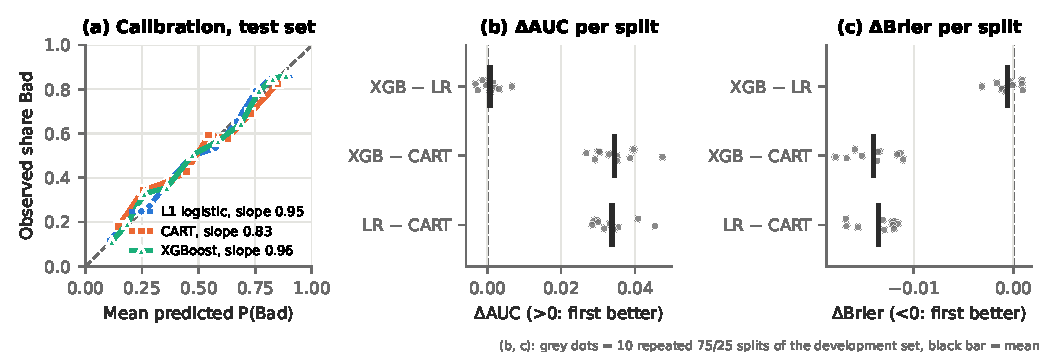
\includegraphics[width=\textwidth]{../results/figures/fig1_predictive.pdf}
\caption{(a) Reliability curves on the final test set (10 quantile bins). (b, c) Paired differences between models within each repeated development split; each split re-runs model selection.}
\label{fig:pred}
\vspace{-3mm}
\end{figure}

\textbf{Predictive accuracy.} Table~\ref{tab:pred} and Fig.~\ref{fig:pred} summarise the comparison. On the final test set, the AUC difference (logistic minus XGBoost) is \dAUCLRXGB{} (95\% interval \dAUCciLRXGB) and the Brier difference is \dBrierLRXGB{} \dBrierciLRXGB; both intervals include zero. Across the \NRepeats{} development splits, with model selection repeated each time, XGBoost's AUC exceeded the logistic model's in \RepAucDiffPosXGBLR{} splits; the mean difference was \RepAucDiffXGBLR{} (range \RepAucDiffMinXGBLR{} to \RepAucDiffMaxXGBLR{}), and XGBoost's Brier score was higher in \RepBrierDiffPosXGBLR{} splits. The depth-limited CART is worse in every comparison, including all \NRepeats{} development splits (test AUC \TestAUCCART{}, logistic minus CART \dAUCLRCART{} \dAUCciLRCART), and its CV score rose monotonically with the depth limit. This suggests that the imposed depth restriction contributed to the gap; our results concern this restricted CART family. All three models are close to calibrated in the large (mean observed minus mean predicted P(Bad): \CITLLR{}, \CITLCART{} and \CITLXGB{} for logistic, CART and XGBoost); the recalibration slopes below one (Table~\ref{tab:pred}) indicate that predictions are somewhat too extreme, most for CART. Similar AUC does not mean similar individual predictions: the logistic model and XGBoost agree on the label at 0.5 for \AgreeLRXGB{} of test applicants, but \GtTenLRXGB{} receive probabilities more than 0.10 apart (mean absolute difference \MeanAbsLRXGB).

\textbf{What the structures show.} The logistic model has \LRnnz{} non-zero coefficients on \LRvars{} of the 23 variables. It can be inspected in full, but 30 terms do not make it readily simulatable by a typical applicant. Inspection shows two signs that run against the dictionary's monotonicity constraints. Relative to ``current and never delinquent'', the odds ratio for a 120+-day worst-ever delinquency (\var{MaxDelqEver}) is \ORMDEOneTwenty{}, and for a 120+-day delinquency in the last 12 months (\var{MaxDelq2PublicRecLast12M}) \ORMDTwelveOneTwenty{}. Odds ratios are per change of the original column, here a dummy from 0 to 1, i.e.\ $\exp(\text{standardised coefficient}/\text{column s.d.})$. Raw Bad rates for the two \var{MaxDelqEver} categories are \BadRateMDEOneTwenty{} (120+ days) and \BadRateMDENever{} (never delinquent). A higher marginal risk with a negative conditional coefficient among correlated delinquency variables is not a statistical contradiction. The dictionary's constraint concerns the model's response, however, and the first sign was negative in \NegMDEOneTwenty{} of \NRuns{} refits. This stable sign motivates a domain and specification audit; it does not by itself establish a modelling error. The tree has depth \CARTdepth{}, \CARTleaves{} leaves and \CARTvars{} variables; every applicant's decision is a path of at most five tests. XGBoost has \XGBtrees{} trees and \XGBleaves{} leaves and uses all \XGBvars{} variables; its structure cannot be inspected in the same way.

\begin{figure}[htbp]
\centering
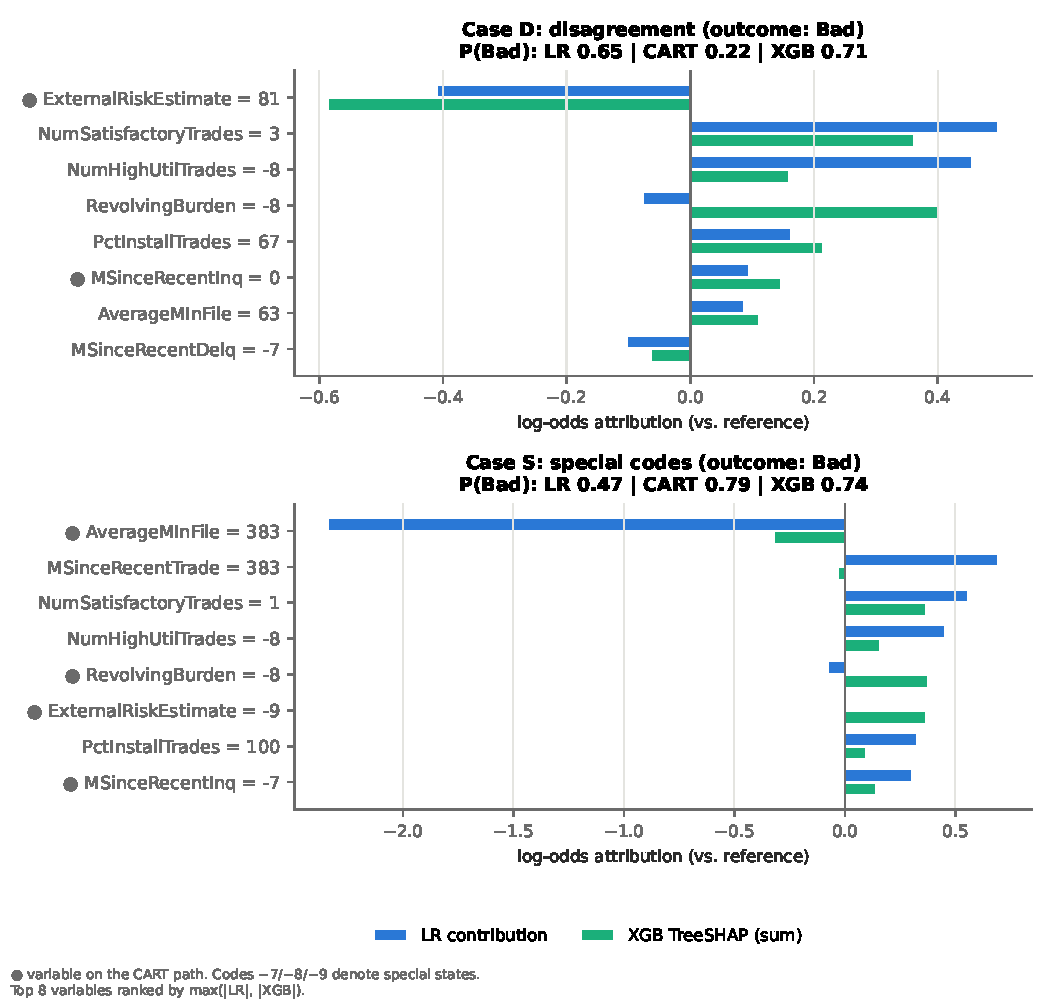
\includegraphics[width=0.94\textwidth]{../results/figures/fig2_cases.pdf}
\caption{Same-case explanations for two pre-selected test applicants, summed per original variable, in log-odds relative to the same 200-row reference sample. Bars: logistic attribution (blue) and XGBoost TreeSHAP (green); the 8 variables shown have the largest $\max(|\text{logistic}|, |\text{TreeSHAP}|)$.}
\label{fig:cases}
\vspace{-3mm}
\end{figure}

\textbf{Same-case explanations} (Fig.~\ref{fig:cases}; all five cases in the supplementary tables). Case~D has the largest disagreement: logistic \CaseDLR{}, XGBoost \CaseDXGB{}, CART \CaseDCART{}. Its tree path tests \var{ExternalRiskEstimate} twice, the age of the oldest trade and the recency of inquiries, and ends in a leaf of \CaseDLeaf{} training applicants. The path is complete and faithful, but it never looks at the low number of satisfactory trades, which both other models treat as a main risk factor. Case~S has \CaseSNSpecial{} special-code states, no \var{ExternalRiskEstimate}, a single trade and \var{AverageMInFile}\,$=$\,\CaseSAvgMInFile{} (the maximum in the data). The logistic model extrapolates linearly, assigning \CaseSLRAvg{} log-odds to that one value, while XGBoost saturates at \CaseSXGBAvg{}. The tree routes \CaseSMissingSplits{} of its \CaseSPathLen{} tests by its learned missing-value direction: a missing bureau score goes to the low-score branch, ``no inquiries'' ($-7$) goes to the ``inquiry within the last month'' branch, and ``no usable revolving trades'' ($-8$) goes to the high revolving-burden branch. These routings are faithful to the model and readable on a single path; XGBoost's default directions can also be inspected, tree by tree, but not as one readable rule. Whether the routings are reasonable is a domain question. Both cases are illustrations, not population evidence.

\begin{figure}[htbp]
\centering
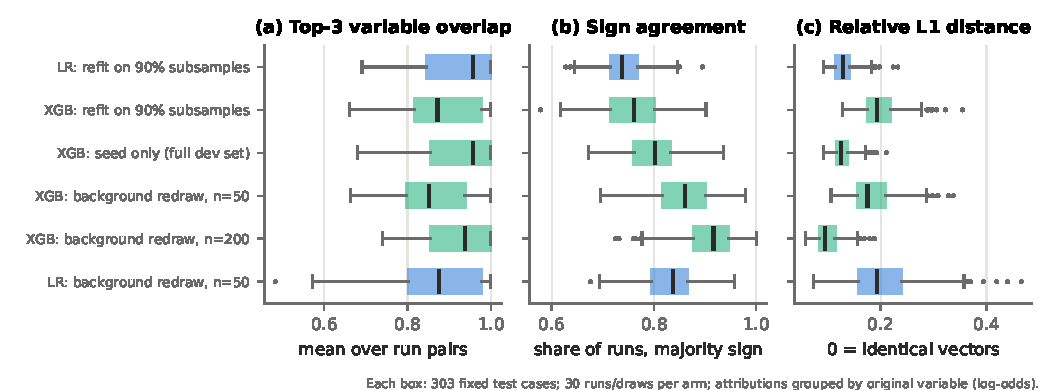
\includegraphics[width=0.94\textwidth]{../results/figures/fig3_stability.pdf}
\caption{Stability of grouped attributions for \NEval{} fixed test cases. Top rows: refits with a new 90\% development subsample and new seed, or new seed only (hyperparameters fixed). Bottom rows: final model fixed, reference sample redrawn.}
\label{fig:stab}
\vspace{-3mm}
\end{figure}

\textbf{Stability} (Fig.~\ref{fig:stab}). Under combined refitting (new subsample and seed), the mean per-case standard deviation of P(Bad) is \PredSDRtLR{} (logistic), \PredSDRtXGB{} (XGBoost) and \PredSDRtCART{} (CART). The label at 0.5 is not unanimous across the \NRuns{} refits for \FlipRtLR{}, \FlipRtXGB{} and \FlipRtCART{} of cases. The tree always splits first on \var{\CARTrootTop} but has \CARTleavesMin{}--\CARTleavesMax{} leaves (path-variable Jaccard index \PathJacRtCART{}). The logistic model keeps between \LRnnzMin{} and \LRnnzMax{} non-zero coefficients; \LRalways{} columns are always selected, \LRsometimes{} only sometimes, and no selected coefficient ever changes sign. Mean top-3 overlap is \TopThreeRtLR{} for logistic attributions and \TopThreeRtXGB{} for TreeSHAP (\TopThreeSdXGB{} when only XGBoost's seed changes). Clear sign reversals affect \ConflictRtLR{} of active variables per case for the logistic model and \ConflictRtXGB{} for XGBoost. Logistic reversals occur almost only in the two one-hot delinquency fields, whose dummies enter and leave the model; most of its lower sign agreement reflects coefficients that L1 zeroes in some refits. With the model fixed, redrawing a 50-row reference moves the XGBoost base value by s.d.\ \BgBaseSDFiftyXGB{} log-odds; top-3 overlap is \TopThreeBgFiftyXGB{} (TreeSHAP) and \TopThreeBgFiftyLR{} (logistic), and \TopThreeBgTwoXGB{} for TreeSHAP at 200 rows. Changing the reference \emph{population} changes the question: for the near-threshold case T, total attribution is \SwapTAll{} relative to all applicants, \SwapTGood{} relative to Good applicants only and \SwapTBad{} relative to Bad applicants only.

\FloatBarrier
\section{Exploratory analysis: removing the upstream risk score}\label{sec:ablation}

\textbf{Why this extension matters.} The full-input comparison asks whether a readable downstream rule can compete with a boosted-tree ensemble on the same information. It does not establish an entirely interpretable credit-assessment process: \var{ExternalRiskEstimate} is itself a consolidated score with undocumented construction in the available material. If much of its predictive work is performed upstream, a simple downstream model can inherit that work without exposing its mechanism. This is a substantive qualification of the interpretation of the original experiment, not an accusation that the input is invalid or leaked.

\textbf{Design and status.} After inspecting the main results, we specified a score-removal extension in \texttt{docs/Protocol.md}. It is explicitly exploratory. We remove \var{ExternalRiskEstimate} and its special-state indicator, leaving \NNoScoreVars{} original variables and \NNoScoreCols{} encoded columns. The modelling population and every development, test and inner-CV customer membership remain unchanged. In particular, exclusion of all-$-9$ records is determined from the full records before score removal. Each of the three families is retuned from the same predefined search space using mean CV Brier, including the same training-only early-stopping procedure for XGBoost. Simply deleting the score at prediction time would not be a meaningful comparison, because a trained model expects its original inputs; fixing its original hyperparameters would also disadvantage a model whose optimal complexity changes with its inputs.

\begin{table}[htbp]
\centering\small
\caption{Exploratory score-removal comparison on the same final-test customers. Each no-score model was independently retuned on development folds. The calibration slope is diagnostic and was not used to alter test predictions.}
\label{tab:ablation}
\begin{tabular}{@{}llrrrr@{}}
\toprule
Model & Inputs & AUC & Brier & Log-loss & Cal. slope \\
\midrule
L1 logistic & Full & 0.792 & 0.1856 & 0.554 & 0.95 \\
L1 logistic & No score & 0.791 & 0.1861 & 0.556 & 0.93 \\
CART & Full & 0.758 & 0.2009 & 0.589 & 0.83 \\
CART & No score & 0.754 & 0.2001 & 0.588 & 0.86 \\
XGBoost & Full & 0.796 & 0.1843 & 0.549 & 0.96 \\
XGBoost & No score & 0.794 & 0.1850 & 0.551 & 0.91 \\
\bottomrule
\end{tabular}

\end{table}

\begin{figure}[htbp]
\centering
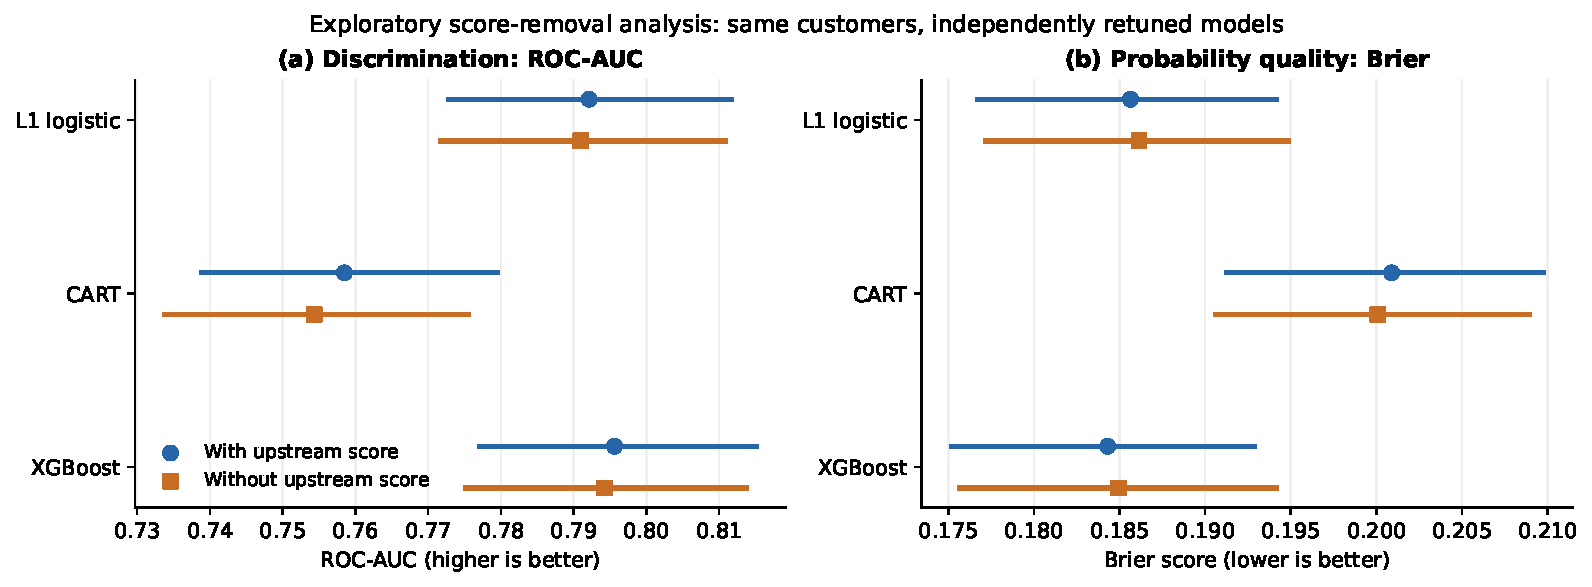
\includegraphics[width=\textwidth]{../results/figures/fig4_ablation_performance.pdf}
\caption{Full versus no-score models. Bars are paired-bootstrap marginal intervals for each model's metric, conditional on its fit. Overlap of these marginal intervals is not the test for a paired difference; see Table~\ref{tab:ablationdiff}.}
\label{fig:ablationperformance}
\end{figure}

\textbf{Aggregate changes.} Without the score, the test AUCs are \NoScoreAUCLR{} for logistic regression, \NoScoreAUCCART{} for CART and \NoScoreAUCXGB{} for XGBoost. The corresponding Brier scores are \NoScoreBrierLR{}, \NoScoreBrierCART{} and \NoScoreBrierXGB{}. Table~\ref{tab:ablationdiff} gives within-family changes using a consistent \emph{full minus no-score} convention: positive AUC changes favour keeping the score, while negative Brier changes favour keeping it. These intervals concern the predictive value of including this input within our learning procedure. They do not estimate a causal effect of the upstream score on default, a benefit of a lending decision, or an intervention on applicants.

\begin{table}[htbp]
\centering\small
\caption{Paired changes from score removal, conditional on the fitted models. Differences are full minus no-score. The comparison is exploratory; no multiplicity-adjusted or equivalence claim is made.}
\label{tab:ablationdiff}
\begin{tabular}{@{}lrr@{}}
\toprule
Model & AUC difference [95\% CI] & Brier difference [95\% CI] \\
\midrule
L1 logistic & \ScoreDeltaAUCLR \ScoreDeltaAUCciLR & \ScoreDeltaBrierLR \ScoreDeltaBrierciLR \\
CART & \ScoreDeltaAUCCART \ScoreDeltaAUCciCART & \ScoreDeltaBrierCART \ScoreDeltaBrierciCART \\
XGBoost & \ScoreDeltaAUCXGB \ScoreDeltaAUCciXGB & \ScoreDeltaBrierXGB \ScoreDeltaBrierciXGB \\
\bottomrule
\end{tabular}

\end{table}

The observed XGBoost-minus-logistic AUC gap is \GapFullXGBLR{} with the score and \GapNoScoreXGBLR{} without it. The observed gap remains small in both settings. This weakens the suggestion that their proximity is \emph{entirely} explained by sharing that one score, but does not show that the score contains no useful information: other bureau variables may substitute for it, and most development splits favour keeping it. All three test AUC-change intervals include zero; this is uncertainty about incremental performance, not a proof of equivalence or a universal property of interpretable models. The no-score logistic model has \NoScoreLRCoef{} non-zero coefficients on \NoScoreLRVars{} original variables; its actual sparsity, rather than the label ``L1'', is what matters for inspection.

\textbf{Development-split evidence.} We repeated the full no-score selection procedure on the same ten development holdouts used for the full-input comparison (Fig.~\ref{fig:ablationrepeated}). Including the score gives a higher AUC in \RepScoreAUCPosLR{} of ten splits for logistic regression, \RepScoreAUCPosCART{} for CART and \RepScoreAUCPosXGB{} for XGBoost. Mean paired AUC changes are \RepScoreAUCMeanLR{}, \RepScoreAUCMeanCART{} and \RepScoreAUCMeanXGB{}, respectively. These are overlapping resamples from one development population. Their spread is a sensitivity description, not a confidence interval based on ten independent studies.

\begin{figure}[htbp]
\centering
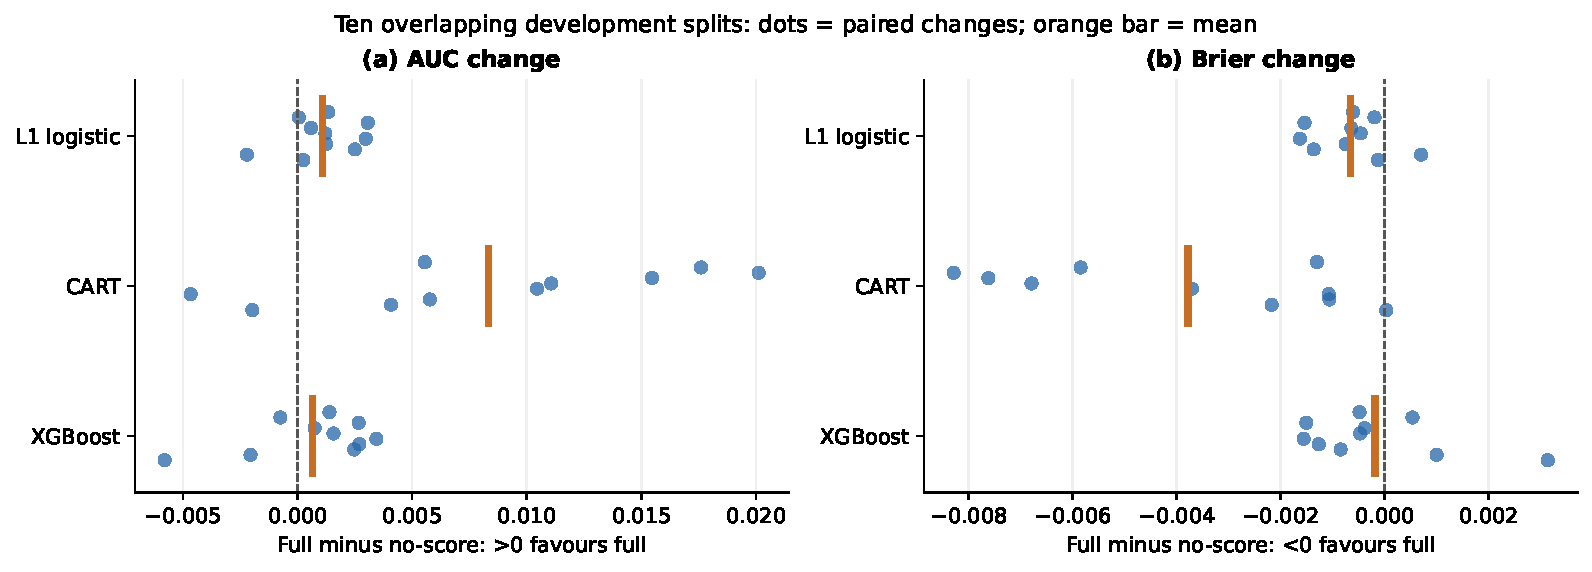
\includegraphics[width=\textwidth]{../results/figures/fig6_ablation_repeated.pdf}
\caption{Effect of score removal within each repeated development split, with both variants retuned on the corresponding training portion. The orange bar is the descriptive mean, not a significance test.}
\label{fig:ablationrepeated}
\end{figure}

\textbf{Individual changes.} Aggregate changes conceal a much larger restructuring of the tree: its AUC change is modest, but nearly half of its customers move by more than 0.10 in predicted risk. This is a comparison of two independently retuned models, not an intervention on one frozen model or on a person. Dropping the score changes predicted default probabilities by more than 0.10 for \NoScoreChangeTenLR{} of test customers under logistic regression, \NoScoreChangeTenCART{} under CART and \NoScoreChangeTenXGB{} under XGBoost (Fig.~\ref{fig:ablationindividual}). Mean absolute changes are \NoScoreMeanChangeLR{}, \NoScoreMeanChangeCART{} and \NoScoreMeanChangeXGB{}. Label disagreement at the descriptive 0.5 threshold is \NoScoreLabelChangeLR{}, \NoScoreLabelChangeCART{} and \NoScoreLabelChangeXGB{}, respectively. Aggregate score changes alone therefore do not describe how the alternative models treat the same recorded applicant. We have no lending-cost model and do not treat 0.5 as an optimal approval threshold.

\begin{figure}[htbp]
\centering
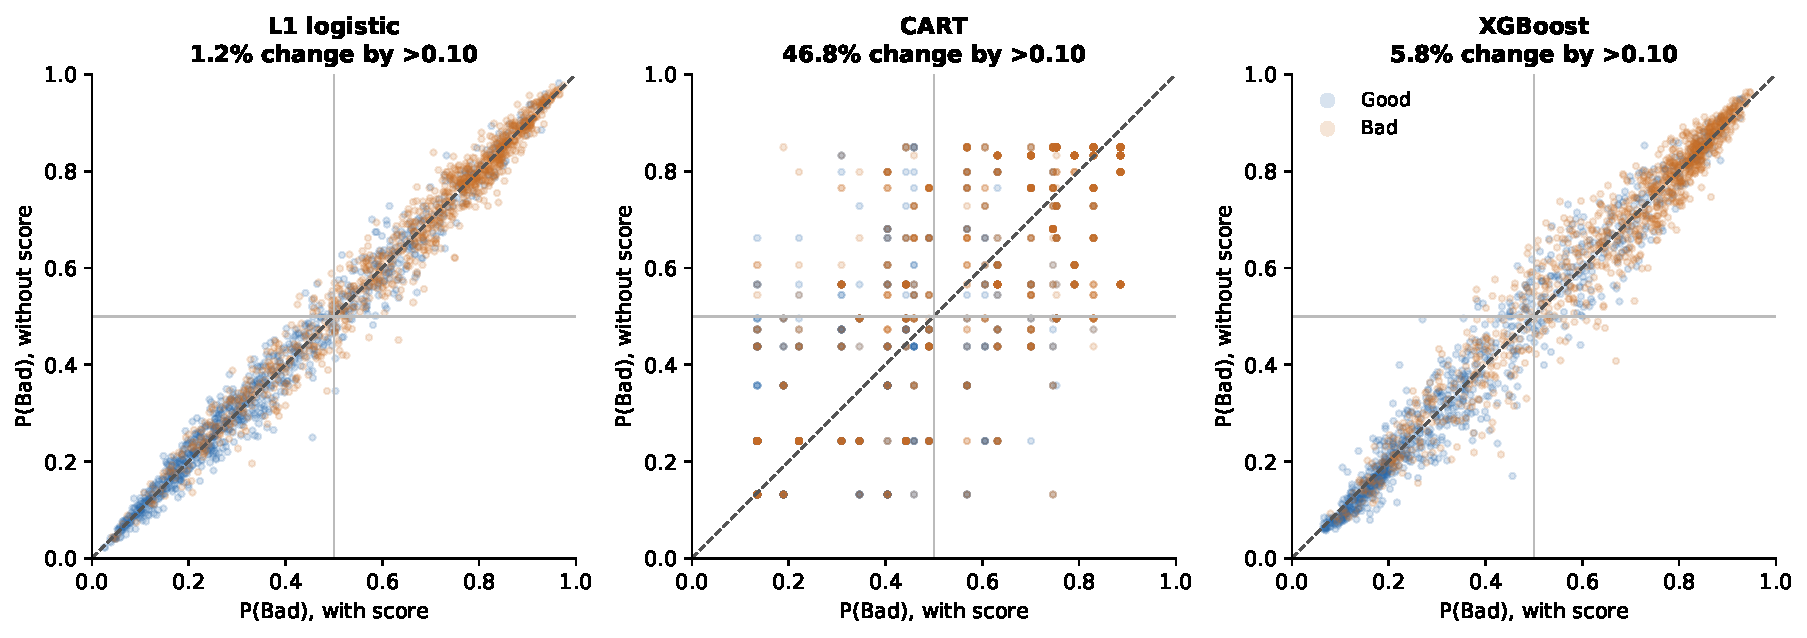
\includegraphics[width=\textwidth]{../results/figures/fig5_ablation_individual.pdf}
\caption{Each point is the same test customer scored by a full and no-score model. Colours denote the observed outcome, not a protected group. Distance from the diagonal indicates a changed probability; crossing a grey line at 0.5 is not evidence of an actual changed lending decision.}
\label{fig:ablationindividual}
\end{figure}

\textbf{Probability validation remains separate.} Figure~\ref{fig:ablationcalibration} shows reliability curves and recalibration slopes for both variants. Brier and log-loss measure overall probability quality, including discrimination and calibration; neither is a pure calibration score. A slope and a binned curve are finite-sample diagnostics, with no formal calibration-equivalence claim. All diagnostics use the models' original predictions, without calibrating them on the test labels.

\begin{figure}[htbp]
\centering
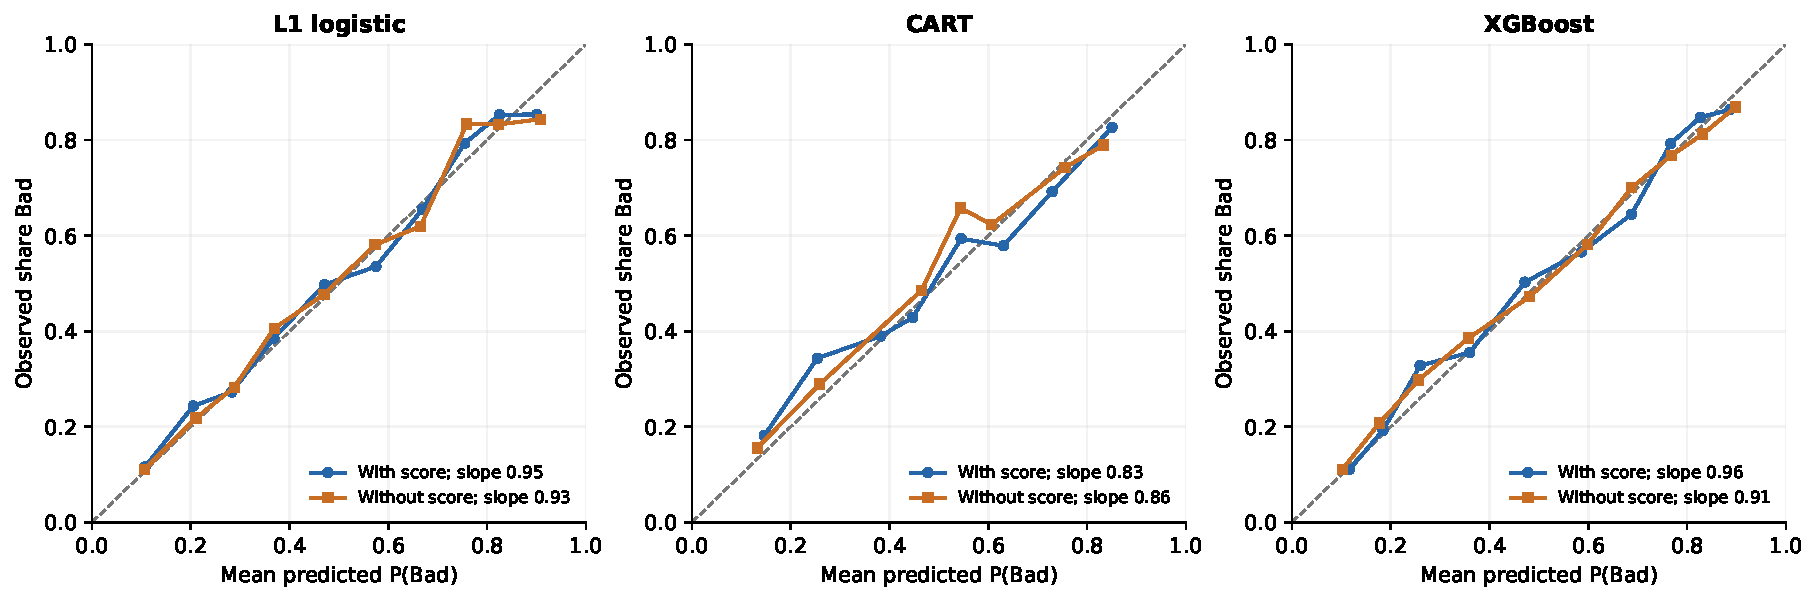
\includegraphics[width=\textwidth]{../results/figures/fig7_ablation_calibration.pdf}
\caption{Calibration diagnostics before and after score removal, using ten quantile bins where distinct predictions permit them. Curves are descriptive estimates on one historical test sample.}
\label{fig:ablationcalibration}
\end{figure}

\textbf{Interpretation limit.} Removing a score cannot remove all information associated with it: the remaining bureau variables may contain overlapping signals, and their own measurement pipeline is only partly documented. The ablation asks about incremental predictive dependence under refitting, not how the upstream score was computed. It also supplies no genuine temporal, institutional or prospective external validation. Thus it sharpens the comparison relevant to Rudin without replacing the validation demanded by Ghassemi et al.

\FloatBarrier
\section{Discussion and limitations}\label{sec:disc}
\textbf{Predictive accuracy.} On this data set the L1 logistic model and tuned XGBoost cannot be separated by AUC or Brier score within our test-set intervals, and across development splits the difference is negligible and changes sign. This is consistent with Rudin's claim for this task. It is not evidence for all high-stakes tasks, and it does not extend to every interpretable model: a depth-5 CART is clearly worse, so the answer depends on which interpretable class is chosen. Equal aggregate accuracy leaves room for many near-optimal models whose individual predictions differ, so the choice among them matters for a given applicant in a way aggregate validation does not reveal.

\textbf{Descriptive accuracy.} The full fitted logistic equation (with its preprocessing) and the tree rules expose the prediction mechanism directly. This computational transparency does not ensure that a shortened explanation, such as a few coefficients or one path, is complete or understandable, and both full-input models inherit the undocumented \var{ExternalRiskEstimate}. TreeSHAP is exactly additive and deterministic, so it is not ``wrong'' about the quantity it defines; but that quantity depends on a reference sample, perturbs features independently, and summarises \XGBleaves{} leaves in 23 numbers. Local attributions of the logistic model depend on the reference too, so reference dependence is a property of attribution, not only of black boxes; the logistic equation and the tree path themselves do not depend on a reference. Transparency did let us see a stable counter-intuitive sign and questionable missing-value routings, in line with Rudin's and Murdoch et al.'s argument that interpretable models make flaws detectable. Seeing a possible flaw does not tell whether it is an error, confounding or a real conditional pattern; that requires validation, as Ghassemi et al.\ argue, for interpretable models too.

\textbf{Relevancy.} An applicant needs a short, contestable account of the main factors. A tree path is one candidate representation; the logistic model's 30 terms must be shortened first, and conditional signs and reference choices must be stated or they mislead. A credit officer needs calibrated probabilities and decisions that are stable near the cut-off, which differ across models in our retraining results. An auditor gains most from global structure, which XGBoost offers only through aggregated attributions plus validation. Without a user study we cannot claim that any explanation improves understanding or decisions.

\textbf{Limitations.} One public data set of uncertain sampling and period. No sensitive attributes are available, so we cannot assess discrimination, and their absence does not show its absence \cite{goodman2017eu}. \var{ExternalRiskEstimate} is an undocumented upstream score used by all full-input models; its removal is examined only in the declared exploratory extension. The data and dictionary are secondary copies. Hyperparameter budgets are moderate and we implemented no richer interpretable model. The selected CART lies at the upper end of two grid ranges (depth 5, by design, and minimum leaf size \CARTminleaf{}), and values beyond them were not explored. Bootstrap intervals are conditional on fitted models, and the repeated splits are dependent. The main retraining arm changes data and seed together, and no arm covers the full set of near-optimal models.

\section{Conclusion}
On the full-input HELOC benchmark, L1 logistic regression and XGBoost have close observed discrimination and overall probability scores, with an uncertain paired difference, while a depth-limited CART is worse. The exploratory removal of the upstream score preserves the observed proximity of the first two models, weakening the suggestion that their proximity is entirely explained by sharing that one score. Yet removal can substantially change individual probabilities, particularly for CART, despite modest aggregate metric changes. The full-input explanation experiments show that reference choice and refitting matter for both linear attributions and TreeSHAP; a readable model can also display stable but questionable behaviour. These findings support seriously considering inspectable alternatives and independently validating every model. They do not establish statistical equivalence, causal explanations, human comprehension, freedom from discrimination or performance in a new deployment population.

\FloatBarrier
\appendix
\section{Reading the evidence through the four papers}\label{app:literature}

\begin{longtable}{@{}>{\raggedright\arraybackslash}p{2.4cm}>{\raggedright\arraybackslash}p{4.35cm}>{\raggedright\arraybackslash}p{8.65cm}@{}}
\toprule
Reading & Claim used in this project & Evidence supplied and remaining boundary \\
\midrule
\endhead
Rudin (2019) & Accurate interpretable alternatives should be seriously attempted in high-stakes structured prediction. & Shared-fold comparison of L1 logistic regression, restricted CART and XGBoost; the no-score extension checks dependence on an undocumented upstream score. These are selected model families, not an exhaustive search over all interpretable models. \\
Murdoch et al. (2019) & Predictive accuracy, descriptive accuracy and audience relevance are distinct desiderata. & AUC/probability diagnostics, explicit equations and paths, additive decompositions and stability checks are reported separately. User understanding and decision quality are not measured. \\
Ghassemi et al. (2021) & A plausible explanation cannot certify the validity of an individual decision; validation remains necessary. & Readable but questionable missing-state routings, conditional coefficient signs and prediction variability motivate further validation. Credit-data evidence does not establish a clinical claim, and internal resampling is not external validation. \\
Goodman and Flaxman (2016/2017) & Algorithmic decisions raise explanation, discrimination and accountability questions. & Inputs, preprocessing, reference populations and limitations are disclosed. No protected attributes are present, so neither absence of discrimination nor legal compliance can be established. \\
\bottomrule
\end{longtable}

The four readings are not four votes for the same deployment policy. In particular, Ghassemi et al. do not argue that simply replacing a black box with a transparent model solves safety. Our empirical contribution is to make those distinctions visible within one reproducible credit-risk example, rather than to settle the entire debate.

\section{What exactly is measured?}

For a recorded customer $x$, a model estimates $p(x)=P(Y=\mathrm{Bad}\mid x)$ under the training distribution. ROC-AUC measures ranking between positive and negative observations. Brier is the mean of $(p_i-y_i)^2$; log-loss penalises incorrect confident probabilities. The latter scores are proper probability scores, but should not be described as calibration alone. Reliability curves compare mean prediction with outcome frequency in bins. Logistic recalibration fits $\operatorname{logit}P(Y=1)=a+b\operatorname{logit}(p)$ as a diagnostic; it is not used to refit the reported test probabilities.

For a linear logit model on its transformed inputs $z$, the reference-centred contribution is $\phi_j=w_j(z_j-E_B[Z_j])$, with base value $b+w^T E_B[Z]$. This reconstructs the logit exactly. Interventional TreeSHAP also reconstructs the chosen raw model output, but assigns contributions under its own feature-coalition/reference definition. Such additivity is a computational property, not a sufficient definition of a good explanation, unique internal reasoning or a causal effect. Dummy and special-state contributions are summed back to original variables for display; this is not recomputing a group Shapley game. Independent perturbations may combine encoded states that are not valid joint customer records.

Top-$k$ overlap in this study is $|T_k^{(r)}\cap T_k^{(s)}|/k$, averaged over pairs of fits or reference draws. It is not Jaccard overlap, which is used separately for sets of variables on CART paths. Sign agreement counts contributions with absolute value below 0.01 log-odds as no stable direction; a selected coefficient becoming zero can lower this measure without becoming negative. The separate sign-conflict measure records variables whose contributions have both clearly positive and clearly negative values across runs. Prediction-label instability means that at least two of the 30 fits lie on different sides of 0.5, not the probability of an incorrect bank decision.

\section{Code availability and reproducibility}
The accompanying code directory contains \texttt{README.md}, \texttt{run\_all.sh}, the locked dependencies, shared configuration, experiment scripts and saved numerical outputs. The raw CSV is retrieved separately and verified against its SHA-256 before loading. Run \texttt{bash run\_all.sh} for the complete experiment, or \texttt{bash run\_all.sh --report-only} to rebuild figures and reports from the included saved results. The latter does not refit models or claim to repeat model-based validation. The full training run includes the model checks and independent numerical checks.

Data source and dictionary limitations are documented in \texttt{data/README.md}. Raw data, environments, caches and fitted model binaries are not included in the GitHub folder. They are recreated locally. Report tables and numerical macros are generated from saved results; class direction, row alignment and probability-output scales are checked explicitly.

\FloatBarrier
{\footnotesize
\bibliographystyle{unsrtnat}
\bibliography{refs}
}
\end{document}
